\documentclass{article}
\usepackage{amsmath}
\usepackage{graphicx}
\usepackage{amssymb}
\usepackage{caption}
\usepackage{subcaption}
\usepackage{float}
\newcommand{\Z}{\mathbb{Z}}

\newcommand{\N}{\mathbb{N}}

\newcommand{\Q}{\mathbb{Q}}

\newcommand{\R}{\mathbb{R}}

\newcommand{\C}{\mathbb{C}}

\title{The Ramifications of High Dimensional Spaces on Machine Learning Techniques}
\author{Jonathan Gryak
\qquad
Michael Iannelli\\
PhD Program in Computer Science\\
CUNY Graduate Center\\
City University of New York\\
\texttt{\{jgryak, miannelli\}@gradcenter.cuny.edu}}
\date{}
\begin{document}

\maketitle

\begin{abstract}
Stuff
\end{abstract}
\tableofcontents
\section{Introduction}
motivation:\\
-nearest neighbor\\
-k-means\\
-similarity indexing\\
need more references for the use of these in high dimensions\\
in the introduction to machine learning book, it speaks of dimensionality with respect to density estimation,
not sure if that's useful here

\

The ``curse of dimensionality" coined by Richard Bellman in 1961\cite{bellman1961adaptive}, comes in many forms, including Bellman's original context of optimization, functional approximation, and combinatorics. In this era of ``big data", ``big" not only refers to the indefatigable increase the amount of data collected, but also in the number of features and components that are utilized in the data analysis. However,  as shown in\cite{aggarwal2001surprising}, the increase in the number of features considered, which are usually considered as a multi-dimensional space, has grave repercussions for machine learning techniques that rely on some measure of distance between points in the feature space. Moreover, in 
\section{Properties of High Dimensional Spaces}
I'm not sure what we should put here. The only reference we have for this part are Haralick's slides.

\
Geometry
-distance between spaces decreases\\
-volume shrinks\\
-shell pushed to boundary\\
-bounding box volume pushed to corners

\
In \cite{aggarwal2001surprising}, the authors investigate this peculiar geometry through the lens of $\mathcal{L}_k$ norms. For $k\in\Z$, the norm of two vectors $x,y\in\R^n$ is defined as
$$
\mathcal{L}_k=\left(\sum_{i=1}^n\|x\|^k\right)^{1/k}.
$$
Note that the limit of this norm is called the $\mathcal{L}_{\infty}$ or max norm, and is defined as
$$
\mathcal{L}_k=\max(|x_1|,\ldots,|x_n|).
$$
The authors make use of a ratio called the \emph{relative contrast}, defined as
$$
\dfrac{Dmax_n^k-Dmin_n^k}{Dmin_n^k},
$$
where $Dmax$ and $Dmin$ are respectively the furthest and closest points to the origin in a data set under the metric induced by $\mathcal{L}_k$. The authors extend work by Beyer\cite{beyer1999nearest} to show that, irrespective of the distribution the points are drawn from, $Dmax_n^k-Dmin_n^k$ increases at a rate of $n^{1/k-1/2}$. This has implications for how each  $\mathcal{L}_k$ performs in high dimensions. Generally speaking, the higher the value of $k$ the less distance can be used to discriminate among points.
\

In addition to 
-accuracy
-fraction metrics
\

In this paper, we wish to experimentally verify these counterintuitive effects. We will perform experiments to determine the effects of dimension, metric choice, and sample size on the distances between points. We will also experiment with drawing points from different distributions. Moreover, we will also explore the effects of these parameters on classification accuracy. 
\section{Experimental Results}
As explained in the previous section, we wish to verify experimentally two effects of high dimension spaces, namely the distance between points and the effect on classification accuracy. 
\subsection{Distance Ratio}
To explore the distance between a set of $K$ points, we focus on the average ratio $r$ of the minimum and maximum distances between all $K$ points. We explore how the following parameters affect $r$:
\begin{itemize}
\item $N$ - the dimension of the space, taking values from $[1,10)\cup[10,20,\ldots,100]$
\item $K$ - the samples space, taking values in $\{5,50,500\}$
\item $L_p$, - the $p-$norm, with $p\in\{1,2,\infty\}$
\end{itemize}
\subsubsection{Uniform Distribution}
In this set of experiments, each of the $N$ components of the $K$ points were drawn from the uniform distribution on the interval $(0,1)$. Figure \ref{fig:exp11} depicts the results for each sample size $K$.
\begin{figure}[H]
    \centering
    \begin{subfigure}[h]{0.45\textwidth}
        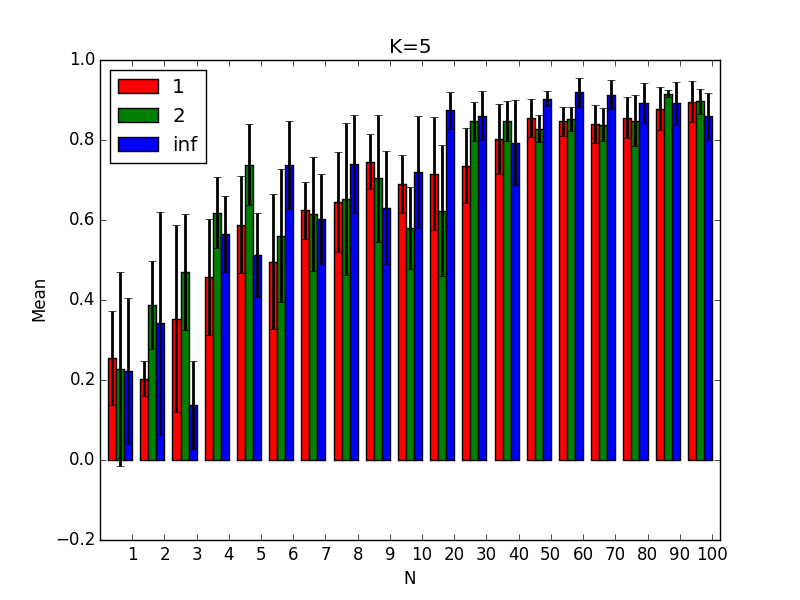
\includegraphics[width=\textwidth]{l-experiment1-1-5-inf.png}
        \caption{$K=5$}
        \label{fig:exp1k5}
    \end{subfigure}
   \begin{subfigure}[h]{0.45\textwidth}
        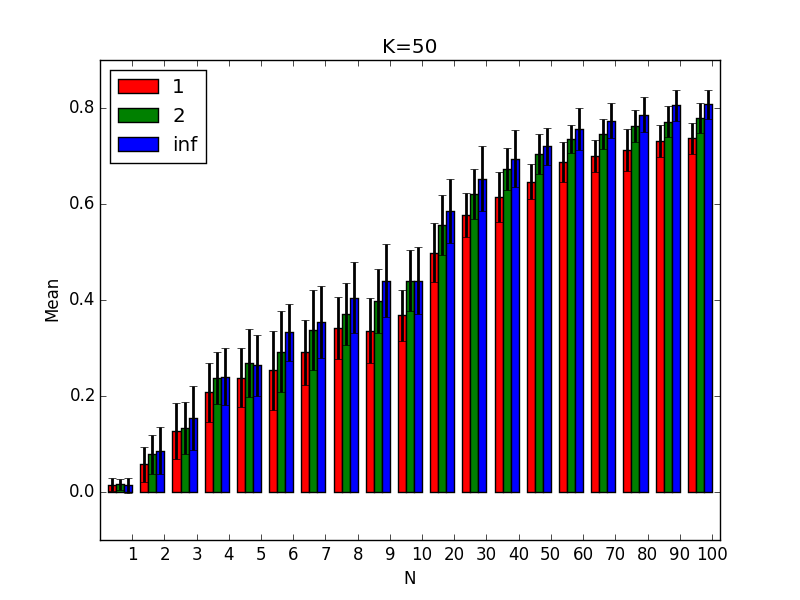
\includegraphics[width=\textwidth]{l-experiment1-1-50-inf.png}
        \caption{$K=50$}
        \label{fig:exp11k50}
    \end{subfigure}
\end{figure}
\begin{figure}[H]
   \centering
   \ContinuedFloat 
    \begin{subfigure}[h]{0.9\textwidth}
        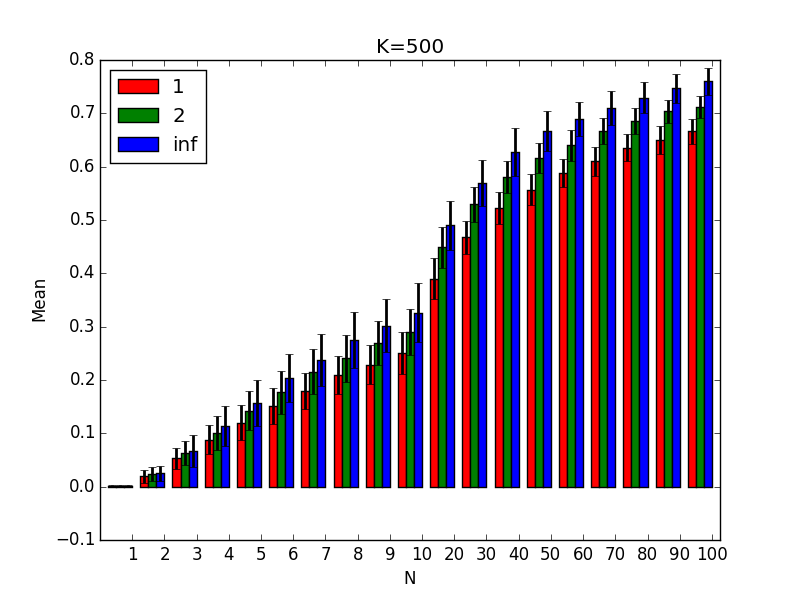
\includegraphics[width=\textwidth]{l-experiment1-1-500-inf.png}
        \caption{$K=500$}
        \label{fig:exp11k500}
    \end{subfigure}
    \caption{Average distance ratio $r$ of $K$ samples for metrics $L_1,L_2,$ and $L_{\infty}$, Uniform Distribution. Standard deviation bars are depicted for each metric and dimension.}\label{fig:exp11}
\end{figure}
As evinced by the large standard deviations, there is a high degree of noise for the smallest sample size ($K=5$),  with no metric being consistently better than the other even as the dimension is increased. However, by $K=50$ a clear trend has formed, with each lower-valued $p$-metric performing better than those with greater value. Notice that the noise of the data has also been reduced. At $K=500$ samples the results are the same, again with less noise that the previous two sample sets.
\
\begin{figure}[H]
\centering
\begin{tabular}{|c|c|c|c|}
\hline
Metric & $N$ & $r$ & \% Difference\\
\hline
1 & 1 & 0.00139 & N/A\\
2 & 1 & 0.00141 & 1.37\%\\
$\infty$ & 1 & 0.00152 & 9.26\%\\
\hline
1 & 10 & 0.25019 & N/A\\
2 & 10 & 0.28958 & 15.74\%\\
$\infty$ & 10 & 0.32590 & 30.26\%\\
\hline
1 & 100 & 0.66599 & N/A\\
2 & 100 & 0.71255 & 6.99\%\\
$\infty$ & 100 & 0.76011 & 14.13\%\\
\hline
\end{tabular}
\caption{Average distance ratios for $K=500$, comparing each norm to $L_1$.}
\label{fig:exp11data}
\end{figure}
In Figure \ref{fig:exp11data}, we see a comparison of the average distance ratios for each metric on the $K=500$ data set. At $N=1$, $r$ is on the order of $10^{-3}$, but by $N=100$, $r$ has grown to approximately .76.
\subsubsection{Normal Distribution}
In this set of experiments, each of the $N$ components of the $K$ points were drawn from a normal distribution with mean 0 and variance 1. The points were normalized using the $\mathcal{L}_2$ norm. Figure \ref{fig:exp2} depicts the results for each sample size $K$.
\begin{figure}[H]
    \centering
    \begin{subfigure}[h]{0.45\textwidth}
        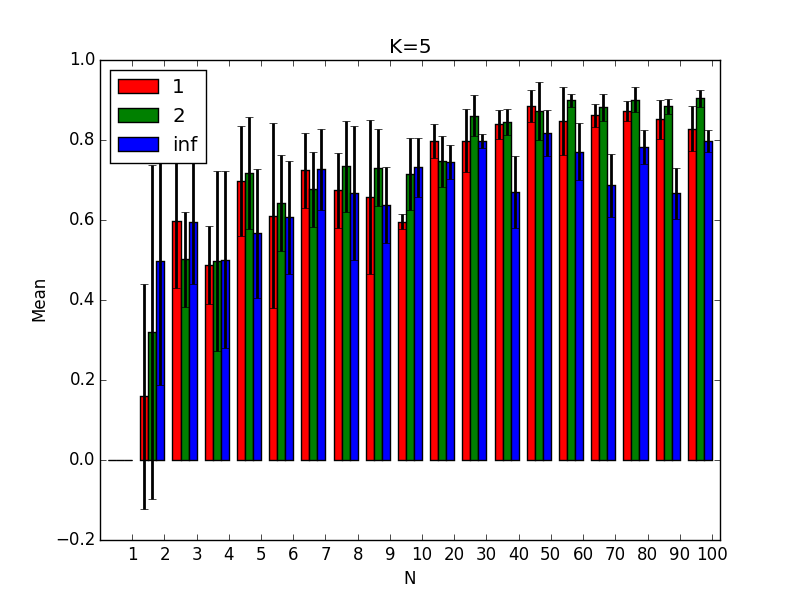
\includegraphics[width=\textwidth]{l-experiment2-5-inf.png}
        \caption{$K=5$}
        \label{fig:exp2k5}
    \end{subfigure}
   \begin{subfigure}[h]{0.45\textwidth}
        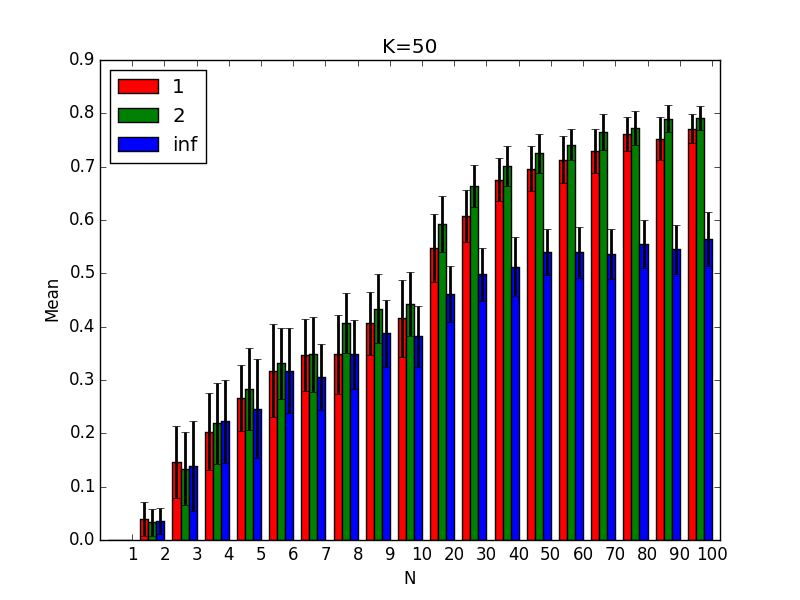
\includegraphics[width=\textwidth]{l-experiment2-50-inf.png}
        \caption{$K=50$}
        \label{fig:exp2k50}
    \end{subfigure}
   \centering
\end{figure}
\begin{figure}[H]
\centering
   \ContinuedFloat 
    \begin{subfigure}[h]{0.9\textwidth}
        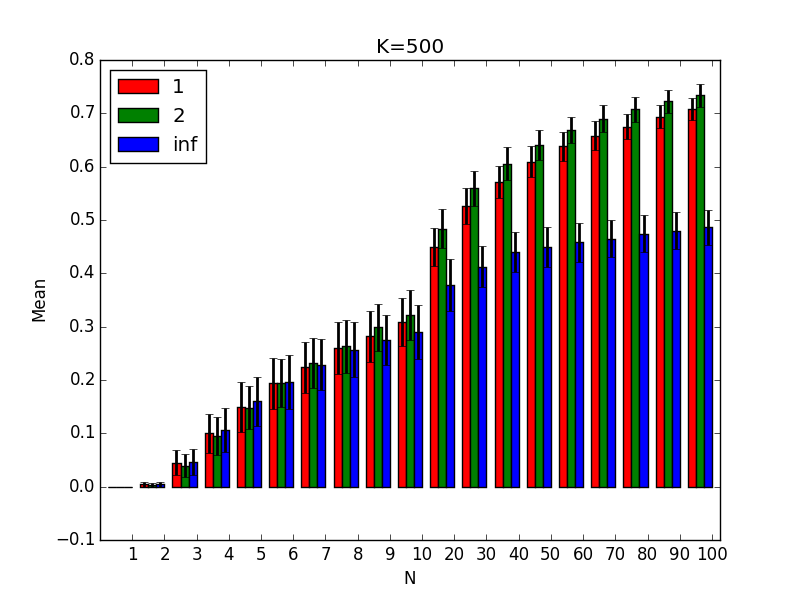
\includegraphics[width=\textwidth]{l-experiment2-500-inf.png}
        \caption{$K=500$}
        \label{fig:exp2k500}
    \end{subfigure}
    \caption{Average distance ratio $r$ of $K$ samples for metrics $L_1,L_2,$ and $L_{\infty}$, normal distribution with mean 0 and variance 1. Standard deviation bars are depicted for each metric and dimension.}\label{fig:exp2}
\end{figure}
As with the uniform distribution, the trend in the performance of the various norms is smoothed as $K$ increases. Also in common with the previous experiment, the $\mathcal{L}_1$ performs better than the $\mathcal{L}_2$ norm. However, it is the $\mathcal{L}_{\infty}$ norm which performs best as $N$ increases.
\

In order to isolate the difference in performance, we first repeated the experiment but varying the normalization. While normalizing using a different norm did change the specific means, it did not change the overall performance. Nor did repeating the experiment without normalization. We then turned our attention to how the $\mathcal{L}_{\infty}$ norm affects points drawn from a uniform or normal distribution differently.
\

For a vector whose components are drawn from a uniform distribution on $(0, 1)$, the $\mathcal{L}_{\infty}$ is bounded by 1, whereas a vector whose components are drawn from a normal distribution arern't bounded, even when the vector is normalized.

Displayed below is the variance of the $\mathcal{L}_{\infty}$ norms on 1000 vectors whose components are randomly drawn from uniform and normal distributions respectively, plotted against the arity of the vector.  The variance decreases to approximately 0 for the uniform distribution, while still remaining relatively high for the normal distribution:
\begin{figure}[H]
\centering
        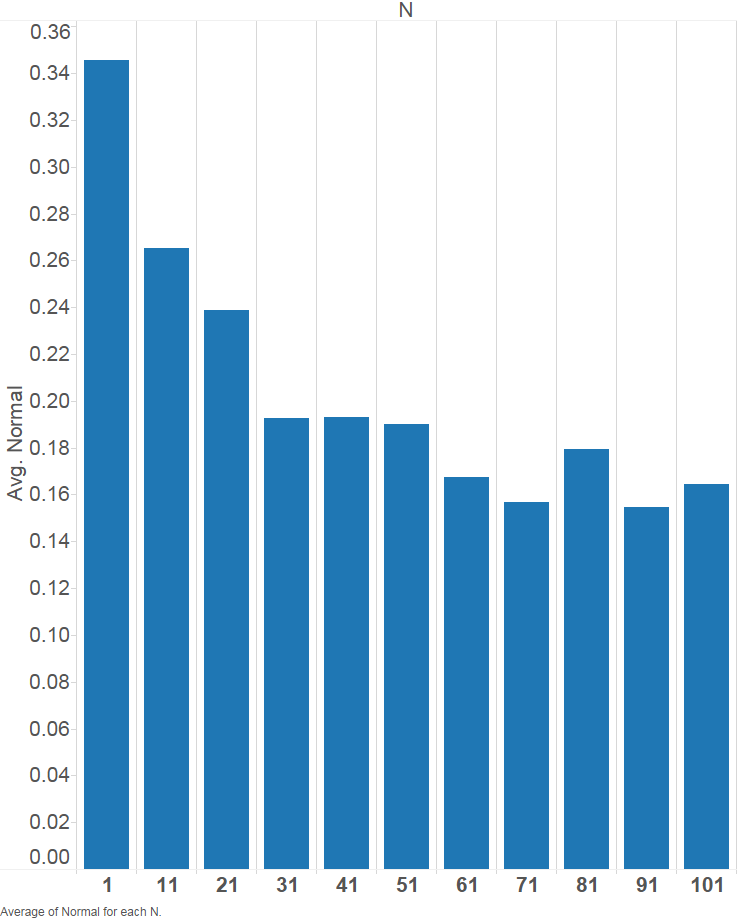
\includegraphics[width=\textwidth]{exp2-var-norm.png}
        \caption{Average Variance of $\mathcal{L}_{\infty}$}
        \label{fig:exp2varnorm}
\end{figure}
From \cite{simlinf}, the $\mathcal{L}_{\infty}$ is good at capturing outlying data. Due to the geometry of high dimensional spaces, outlying values become the defining points of our data. This, combined with the variance of $\mathcal{L}_{\infty}$ of vectors drawn from the normal distributions, may explain these counterintuitive results.

\subsection{Classification Accuracy}
\paragraph{}
In \cite{aggarwal2001surprising}, the impact of different norms on classification accuracy was investigated, where it was demonstrated that, with respect to a random classification, lower valued norms performed better. In this section, we investigate how classification accuracy varies with respect to dimension, sample size, and and data variance. The parameters used in these experiments are:
\begin{itemize}
\item $N$ - the dimension of the space, taking values from $[1,10)\cup[10,20,\ldots,100]$
\item $K$ - the samples space, taking values in $\{10,300\}$ in increments of 10
\item $M$ - the number of points in the data set to be classified
\item $\sigma$ - the standard deviation of a normal distribution, with $\sigma\in\{.05,.1,.15,.2,.25\}$
\end{itemize}
\paragraph{}
For each experiment, a labeled set $X$ of $K$ $N$-dimensional sample points was generated, with the component of each point being drawn from a uniform distribution on $(0,1)$, and each point being assigned a random, binary classification (i.e., 0 or 1). Then, a data set $Y$ of $M$ $N$-dimensional points is generated with components drawn  from a uniform distribution on $(0,1)$. Each point in $Y$ is given the classification by it nearest neighbor in $X$. The new dataset $\tilde{Y}$ is created by taking each point in $Y$ and perturbing each of its components by adding a value drawn from a normal distribution with mean $0$ and variance $\sigma$. The dataset $\tilde{Y}$ is then classified in the same way as $Y$, and the confusion matrix of between $Y$ and $\tilde{Y}$ is then generated.
For each combination of $N$, $K$, and $\sigma$ values, ten trials of the above experiment were performed. The results of the trials were then averaged. The standard Euclidean norm ($\mathcal{L}_2$) was used in all experiments throughout this section. Note that we also used a different measure of accuracy than in \cite{aggarwal2001surprising}. Accuracy in this section is defined as:
$$
	\dfrac{\#\textrm{true positives}+\#\textrm{true negatives}}{\#\textrm{total outcomes}}
$$
\subsubsection{The Effect of Dimension on Accuracy}
\begin{figure}[H]
    \centering
        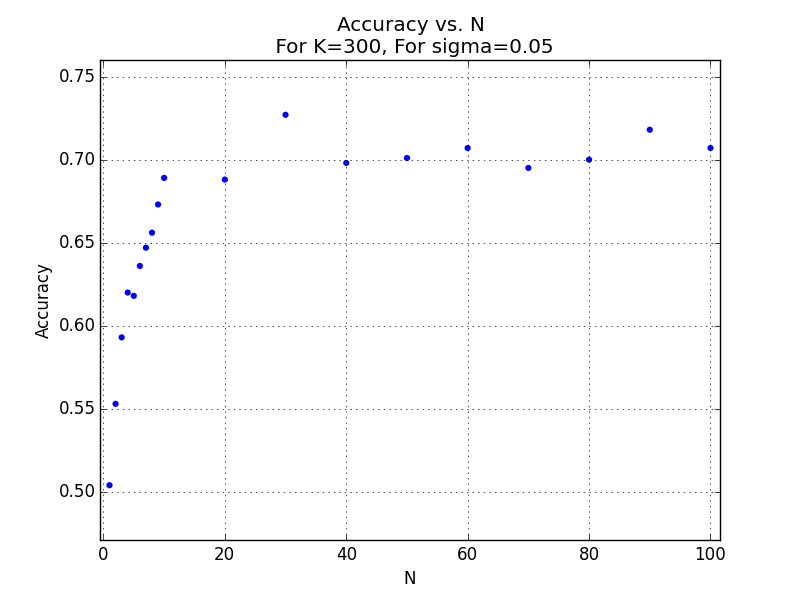
\includegraphics[width=\textwidth]{l-experiment1-2-accuracy-n-k-300-s-005.png}
    \caption{Accuracy as $N$ Varies, $K=300$, $\sigma=.05$}\label{fig:exp1-2-accuracy-n}
\end{figure}
\begin{figure}[H]
\centering
\begin{tabular}{|c|c|c|c|}
\hline
$N$&\multicolumn{2}{|c|}{Confusion Matrix}&Accuracy\\
\hline
1&27.9&24.7&0.504\\
\cline{2-3}
&24.9&22.5&\\
\hline
10&35.8&13.9&	0.689\\
\cline{2-3}
&17.2&33.1&\\
\hline
100&35&14.1&0.707\\
\cline{2-3}
&15.2&35.7&\\
\hline
\end{tabular}
\caption{Confusion Matrices for Figure \ref{fig:exp1-2-accuracy-n}}\label{fig:cm-exp1-2-accuracy-n}
\end{figure}
Our experiments showed a positive relationship between accuracy and dimension. From the results depicted in Figures \ref{fig:exp1-2-accuracy-n} and \ref{fig:cm-exp1-2-accuracy-n}, we see that accuracy starts at approximately 50\%, climbs rapidly to approximately 70\%, the remains at that level as the number of dimensions increases. Lower samples size and higher variance increased the amount of noise in the data but did not produce contradicting results.
\subsubsection{The Effect of Sample Size on Accuracy}
\begin{figure}[H]
    \centering
    \begin{subfigure}[h]{0.45\textwidth}
        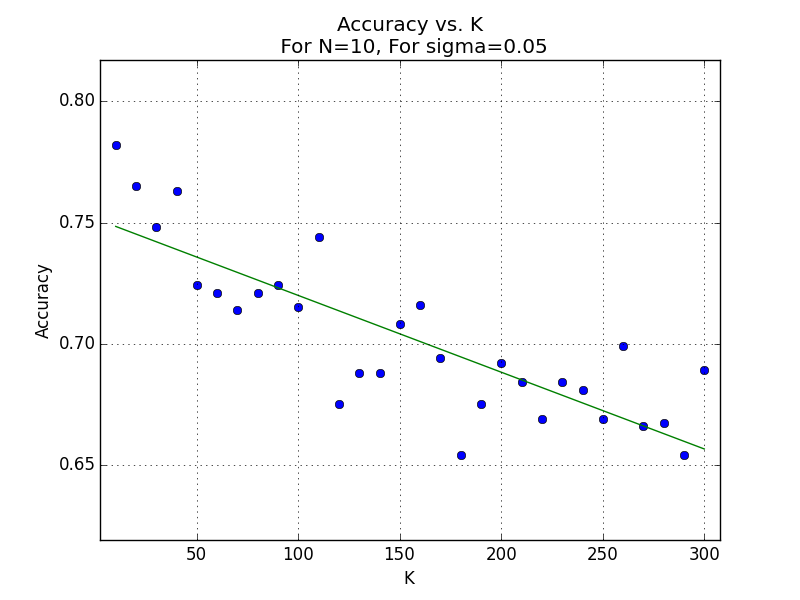
\includegraphics[width=\textwidth]{l-experiment1-2-accuracy-k-n-10-s-005.png}
        \caption{$N=10$}
        \label{fig:exp2k1}
    \end{subfigure}
   \begin{subfigure}[h]{0.45\textwidth}
        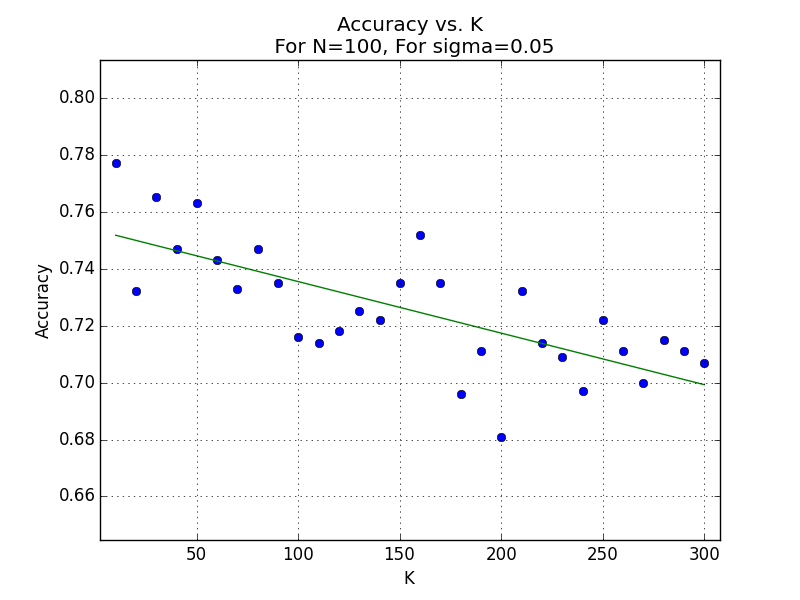
\includegraphics[width=\textwidth]{l-experiment1-2-accuracy-k-n-100-s-005.png}
        \caption{$N=100$}
        \label{fig:exp2k2}
    \end{subfigure}
    \caption{Accuracy as $K$ Varies, $N$ as labeled, $\sigma=.05$}\label{fig:exp1-2-accuracy-k}
\end{figure}
\begin{figure}[H]
\centering
\begin{tabular}{|c|c|c|c|}
\hline
$K$&\multicolumn{2}{|c|}{Confusion Matrix}&Accuracy\\
\hline
10&47.3&12.9&0.777\\
\cline{2-3}
&9.4&30.4&\\
\hline
100&32.8&15.6&0.716\\
\cline{2-3}
&12.8&38.8&\\
\hline
300&35&14.1&0.707\\
\cline{2-3}
&15.2&35.7&\\
\hline
\end{tabular}
\caption{Confusion Matrices for Figure \ref{fig:exp1-2-accuracy-k}}\label{fig:cm-exp1-2-accuracy-k}
\end{figure}
Our experiments showed a negative relationship between accuracy and sample size, which weakened as $N$ increased. In Figure \ref{fig:exp2k1} for $N=10$ we see a drop by .10 in the accuracy over the range of $K$, whereas in figure {fig:exp2k2} for $N=100$ the same range in sample size exhibits only half that reduction in accuracy.
\subsubsection{The Effect of Perturbation Variance on Accuracy}
\begin{figure}[H]
    \centering
        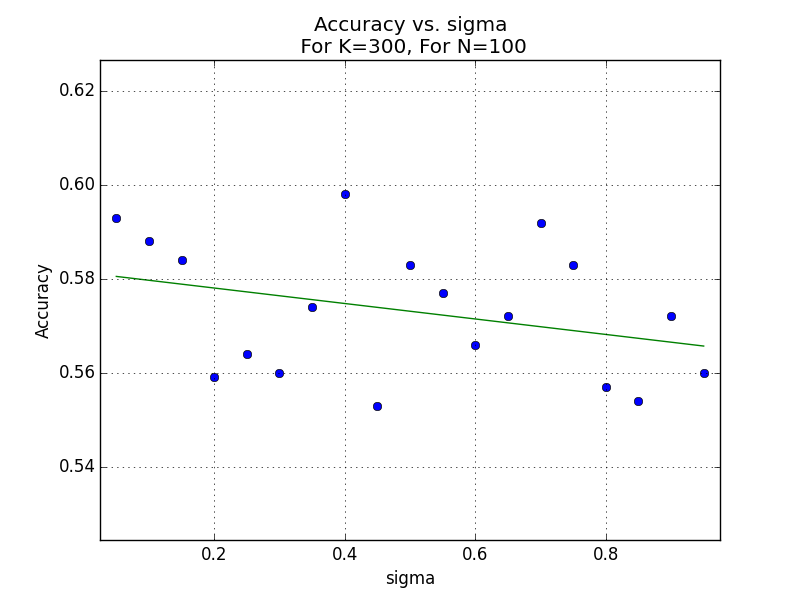
\includegraphics[width=\textwidth]{experiment1-2-sigmas.png}
    \caption{Accuracy as $\sigma$ Varies, $N=100$,$K=300$}\label{fig:exp1-2-accuracy-s}
\end{figure}
Our initial range of $\sigma$  did not reveal any significant correlation with accuracy, so the range of $\sigma$ was expanded from .05  to .95 inclusively in .05 increments, keeping $N$ and $K$ constant at 100 and 300 respectively. As before, 10 trials were run for each $\sigma$ value, and the results for each were averaged. Even in this expanded range, the accuracy oscillated as $\sigma$ increased, staying with a range of .56 to .60.
\subsubsection{On the Number of Classes and Accuracy}
In order to discern the effect of the number of classes on accuracy, we performed additional experiments using class sets of varying cardinality:
\begin{figure}[H]
    \centering
        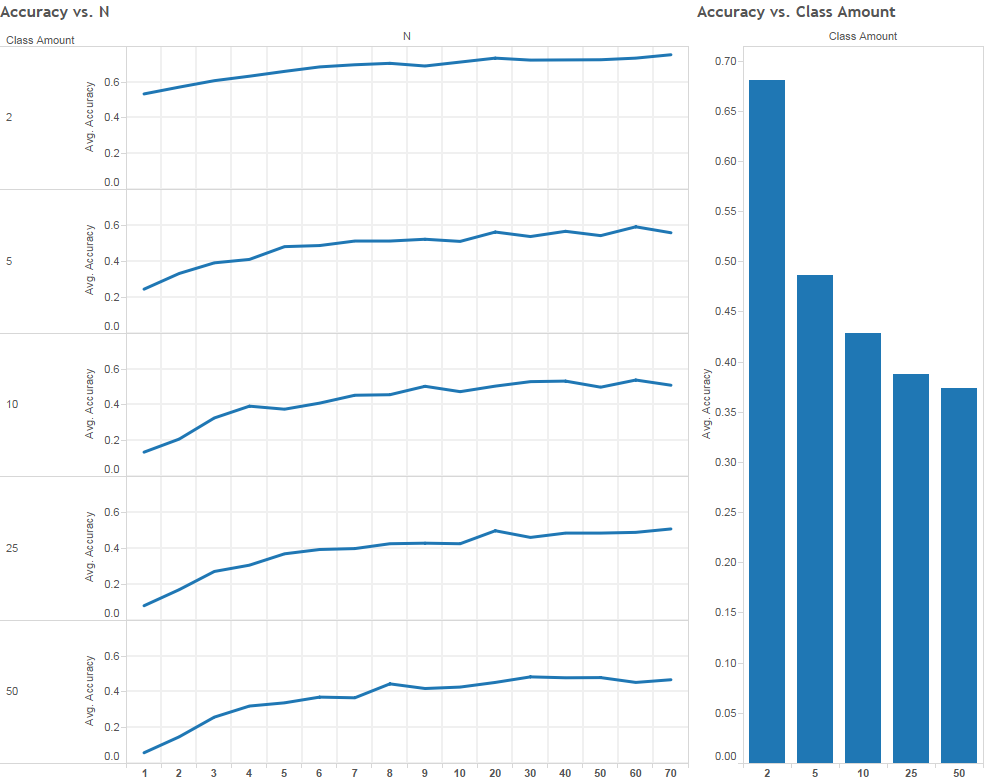
\includegraphics[width=\textwidth]{exp1-2-varying_classes.png}
    \caption{Accuracy as Class Sets are Varied}\label{fig:exp1-2-varclass}
\end{figure}
In the left half of Figure \ref{fig:exp1-2-varclass}, we see that the positive correlation between accuracy and dimension is preserved from the binary classification experiments, albeit with lower overall accuracy. This trend is demonstrated in the left half of the figure. The data suggest that the relatively high accuracy in the original binary classification is due to the proximity of points in high dimensional space, coupled with a paucity of classification choices.
\section{Conclusion}
In conclusion, we have demonstrated that the geometry of high dimensional space greatly impacts the performance of machine learning techniques like near neighbors, that rely upon spatial proximity for their results. The distance between points becomes a poor discriminant in these spaces. We have seen that both the distribution of points as well as the metric used must be considered. We have seen that classification accuracy is effected by the dimension of the space as well as the number of classes used in assignment.
\

Future experiments may investi
-suggest other experiments (fractional distance metric, other clustering, other ML techniques which use distance?
	
\bibliographystyle{plain}
\bibliography{ml-midterm}

\end{document}  